\section{Struttura di una CNN}
L'architettura di una rete neurale convoluzionale è meticolosamente progettata per 
estrarre caratteristiche (o features) significative da dati visivi complessi. 
Ciò è possibile tramite l'uso di livelli specializzati all'interno dell'architettura di rete.
Un CNN presenta la seguente struttura:
\begin{figure}[H]
    \centering
    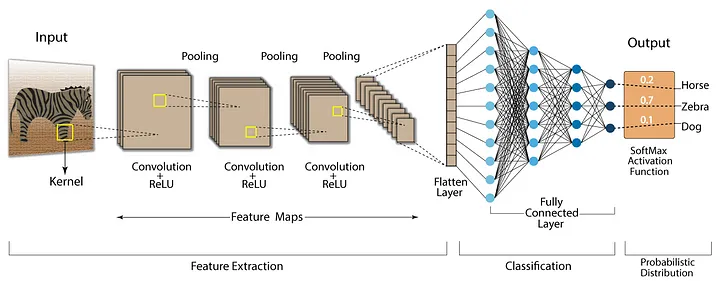
\includegraphics[width=1\textwidth]{Immagini/Generiche/CNN_struttura2.png}
    \caption{Esempio della struttura di un CNN \cite{ELEMENTI_CNN_1}}
    \label{fig:strutturaCNN}
\end{figure}

Come si può osservare, la rete di una CNN è costituita da due blocchi principali: I blocco 
della \textit{features extraction} (estrazione delle caratteristiche), responsabile dell'estrazione 
di tutte le caratteristiche e pattern dell'immagine; E il blocco della classification (classificazione), 
che si occupa di processare tutte le features map (mappe delle caratteristiche) create dal blocco 
precedente e predire il risultato di ogni classe 
\cite{ELEMENTI_CNN_1, ELEMENTI_CNN_2, ELEMENTI_CNN_3}.

All'interno del blocco estrazione delle features sono presenti i seguenti layer:
\begin{itemize}
    \item \textbf{Input Layer}: Esso è il primo layer ed è quello che riceve l’immagine, 
    ed eventualmente, la ridimensiona prima di passarla ai layer successivi.

    \item \textbf{Convolutional Layer}: Questo layer si occupa di estrarre le features, ovvero 
    le caratteristiche significative delle immagini. In pratica si cercano di individuare 
    dei pattern, come ad esempio curve, angoli, circonferenze o quadrati raffigurati in un’immagine con elevata precisione.
    I livelli convolutivi possono essere molteplici ma questo dipende dall'architettura di
    rete: maggiore è il loro numero, maggiore è la complessità delle caratteristiche che
    riescono ad individuare.

    \item \textbf{Activation Layer}: Questo layer viene usato sempre dopo un
    layer convoluzionale. Questo layer consiste nell'applicazione, su singolo pixel, della funzione
    di attivazione, tipicamente la ReLU, permettendo così di introdurre \textbf{non linearità} nella rete. 
    %In oltre, la ReLU permette di sostituire ogni valore negativo con il valore zero.
    
    \item \textbf{Pooling Layer}: Questo livello viene utilizzato per rendere il set di features map 
    piccolo e gestibile riducendo il numero di parametri sulla rete e di conseguenza 
    ottimizzando la computazione; rende inoltre la rete invariante alle piccole trasformazioni quali distorsione o traslazione
    rispetto all’immagine iniziale. Questa operazione permette anche di preservare le 
    informazioni fondamentali.

\end{itemize}

All'interno di una CNN, i layer di convoluzione e di pooling, posso ripetersi più volte. 
Inoltre, 
ci possono essere  molteplici layer convoluzionali in sequenza prima di un layer di pooling. 
% Ma questo dipende dall'architettura di rete: maggiore è il loro numero, maggiore è la 
% complessità delle caratteristiche che riescono ad individuare.

Per quanto riguarda il blocco della classificazione,esso è solitamente posto alla fine 
della rete e si occupa di prendere le immagini filtrate ad alto livello e tradurre in 
categorie ciò che ha analizzato, quindi il suo scopo è
quello di usare le features per classificare le immagini. Ogni classe rappresenta una
possibile risposta finale che il computer darà.
Tipicamente si tratta di un MultiLayer Perceptron che usa alla fine una funzione di 
attivazione \textbf{Softmax}.

\newpage
\section{Algoritmi di Pooling}
Nell’architettura di una CNN è pratica comune inserire degli strati di Pooling, 
la cui funzione è quella di ridurre la dimensione
spaziale degli input (larghezza e altezza), in modo da diminuire il numero di parametri e
il carico computazionale \cite{ELEMENTI_CNN_1, ELEMENTI_CNN_2, ELEMENTI_CNN_3} . 

\subsection{Average-Pooling}

L'\textit{Average-Pooling} consiste nel calcolare la 
media degli elementi presenti nella regione della feature map coperta dal filtro. 
\begin{figure}[H]
    \centering
    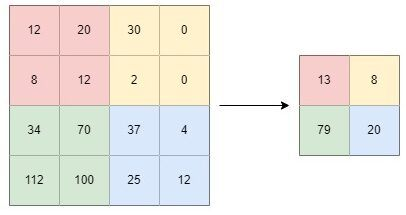
\includegraphics[width=0.5\textwidth]{Immagini/Generiche/avgPool.png}
    \caption{Esempio di un Average-Pooling \cite{PULLING}.}
    \label{fig:avgPool}
\end{figure}

\subsection{Max-Pooling}
Il \textit{Max pooling} è un'operazione di pooling che seleziona l'elemento 
massimo dalla regione della feature map coperta dal filtro. Quindi, 
l'output dopo il layer di max-pooling sarebbe una feature map 
contenente le feature più importanti della feature map precedente.

\begin{figure}[H]
    \centering
    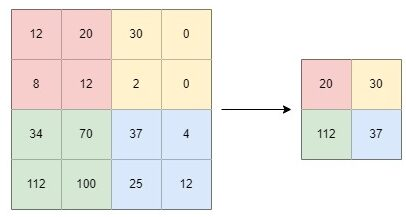
\includegraphics[width=0.5\textwidth]{Immagini/Generiche/maxPool.png}
    \caption{Esempio di un Max-Pooling \cite{PULLING}.}
    \label{fig:maxPool}
\end{figure}

